
\begin{center}
\thispagestyle{empty}

\vspace{1.5cm}

% 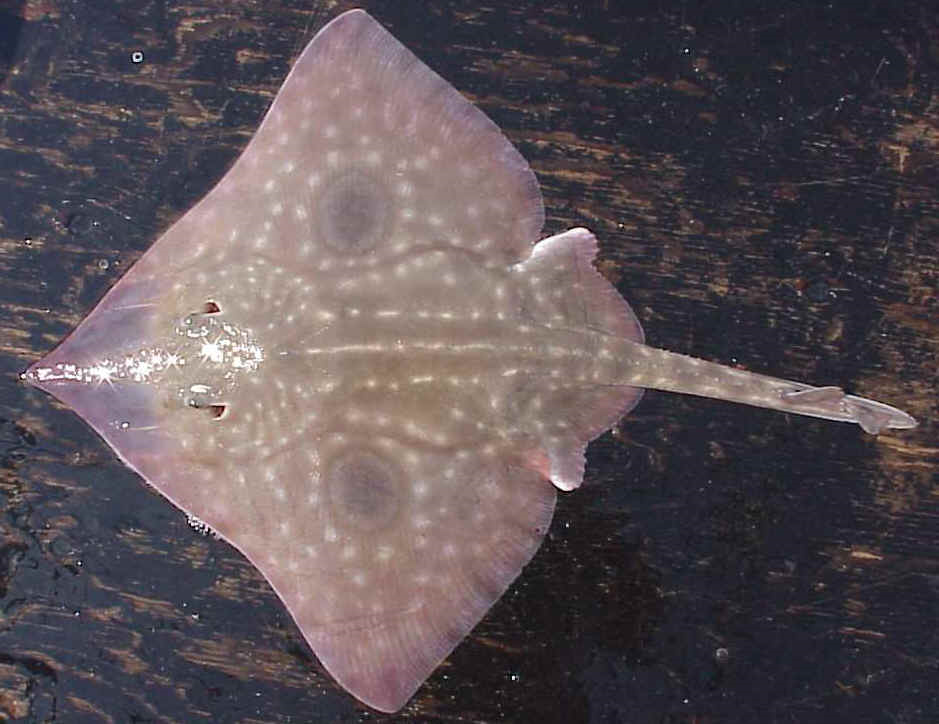
\includegraphics{cover_photo}~\\[1cm]
\pdftooltip{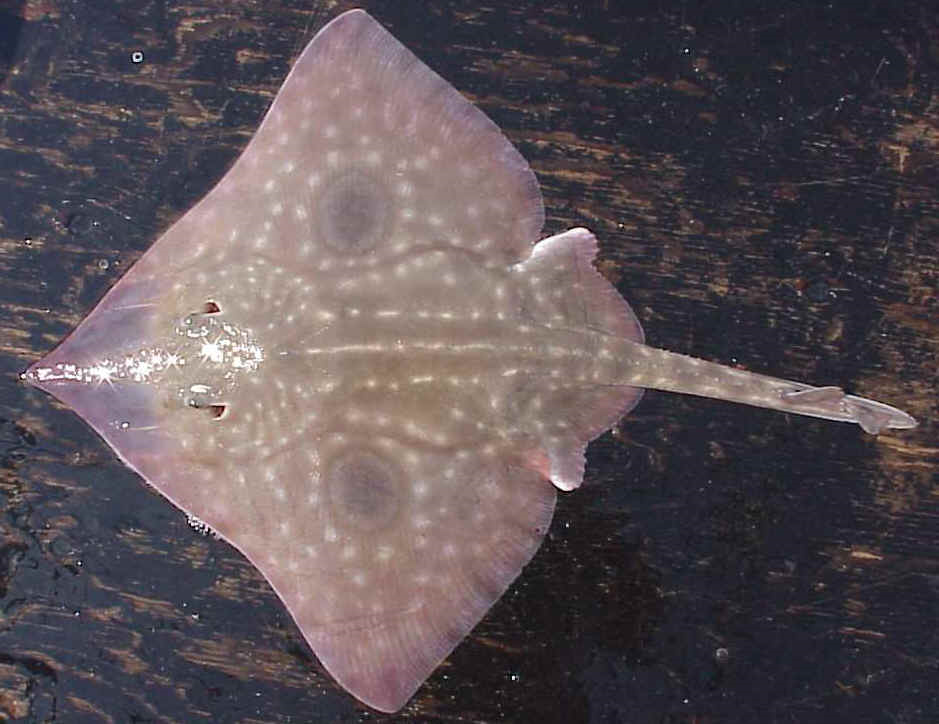
\includegraphics{cover_photo}}{This is a fish.}

\vspace{2cm}

Ian G. Taylor\textsuperscript{1}\\
Vladlena Gertseva\textsuperscript{1}\\
Andi Stephens\textsuperscript{2}\\
Joseph Bizzarro\textsuperscript{3}\\

\vspace{2cm}
\mbox{}

\vspace*{\fill}
\small

\textsuperscript{1}Northwest Fisheries Science Center, U.S. Department of Commerce, National Oceanic and Atmospheric Administration, National Marine Fisheries Service, 2725 Montlake Boulevard East, Seattle, Washington 98112\\

\vspace{.3cm}

\textsuperscript{2}Northwest Fisheries Science Center, U.S. Department of Commerce, National Oceanic and Atmospheric Administration, National Marine Fisheries Service, 2032 S.E. OSU Drive Newport, Oregon 97365

\vspace{.3cm}

\textsuperscript{3}Southwest Fisheries Science Center, U.S. Department of Commerce, National Oceanic and Atmospheric Administration, National Marine Fisheries Service, 110 Shaffer Road, Santa Cruz, California 95060\\



\vspace{.5cm}

\vfill


\vspace{.3cm}
%Bottom of the page
%{\large \today}


\newpage{\thispagestyle{empty}}

\vspace*{\fill}
\begin{flushleft}
This report may be cited as:

Taylor, I.G., Gertseva, V., Stephens, A. and Bizzarro, J. Status of Big Skate (\emph{Beringraja binoculata}) Off the U.S. West Coast, 2019. Pacific Fishery Management Council, Portland, OR. Available from http://www.pcouncil.org/groundfish/stock-assessments/
\end{flushleft}

\newpage{\thispagestyle{empty}}

% Create this table using the instructions in Acronyms.Rmd


\begin{flushleft}
\large{\textbf{Acronyms used in this Document}}
\end{flushleft}

\vspace{.5cm}

\renewcommand{\arraystretch}{1.2}

\begin{table}[ht]
% \centering
\begin{tabular}{rll}
\hline
 &  ABC & Allowable Biological Catch \\ 
 &  ACL & Annual Catch Limit \\ 
 &  AFSC & Alaska Fisheries Science Center \\ 
 &  CDFW & California Department of Fish and Wildlife \\ 
 &  DFO & Canada's Department of Fisheries and Oceans \\
 &  DW & Disk Width \\
 &  IFQ & Individual Fishing Quota \\
 &  IPHC & International Pacific Halibut Commission \\
 &  ISW & Interspiracular Width \\
 &  NMFS & National Marine Fisheries Service \\
 &  NWFSC & Northwest Fisheries Science Center \\
 &  ODFW & Oregon Department of Fish and Wildlife \\
 &  OFL & Overfishing Limit \\
 &  OY & Optimum Yield \\
 &  PacFIN & Pacific Fisheries Information Network \\
 &  PFMC & Pacific Fishery Management Council \\
 &  SPR & Spawning Potential Ratio \\
 &  SSC & Scientific and Statistical Committee \\
 &  SWFSC & Southwest Fisheries Science Center \\
 &  TL & Total Length \\
 &  VAST & Vector Autoregressive Spatio-Temporal Package \\
 &  WCGBT & West Coast Groundfish Bottom Trawl Survey \\
 &  WCGOP & West Coast Groundfish Observer Program \\
 &  WDFW & Washington Department of Fish and Wildlife \\
   \hline
\end{tabular}
\end{table}

\renewcommand{\arraystretch}{1}

\maketitle

\pagenumbering{roman}
\setcounter{page}{1}
\end{center}


